\documentclass{beamer}
%
% Choose how your presentation looks.
%
% For more themes, color themes and font themes, see:
% http://deic.uab.es/~iblanes/beamer_gallery/index_by_theme.html
%
\mode<presentation>
{
  \usetheme{default}      % or try Darmstadt, Madrid, Warsaw, ...
  \usecolortheme{crane} % or try albatross, beaver, crane, ...
  \usefonttheme{structurebold}  % or try serif, structurebold, ...
  \setbeamertemplate{navigation symbols}{}
  \setbeamertemplate{caption}[numbered]
} 

\usepackage[english]{babel}
\usepackage[utf8x]{inputenc}

\title[ML]{Machine Learning}
\author{Pawel Wocjan}
\institute{University of Central Florida}
\date{Fall 2020}

\begin{document}

\begin{frame}
  \titlepage
\end{frame}

% Uncomment these lines for an automatically generated outline.
%\begin{frame}{Outline}
%  \tableofcontents
%\end{frame}

\begin{frame}{Linear Regression}
\begin{itemize}
\item Consider the following toy example.

\medskip
\item It has been known that crickets (an insect species) chirp more frequently on hotter days than on cooler days. 

\medskip
\item Professional and amateur scientists have cataloged data on chirps-per-minute and temperature. 
    
\medskip
\item Using this data, you want to explore this relationship.
\end{itemize}
\end{frame}

%%%

\begin{frame}{Linear Regression}
\begin{itemize}
\item First, examine your data by plotting it:
    
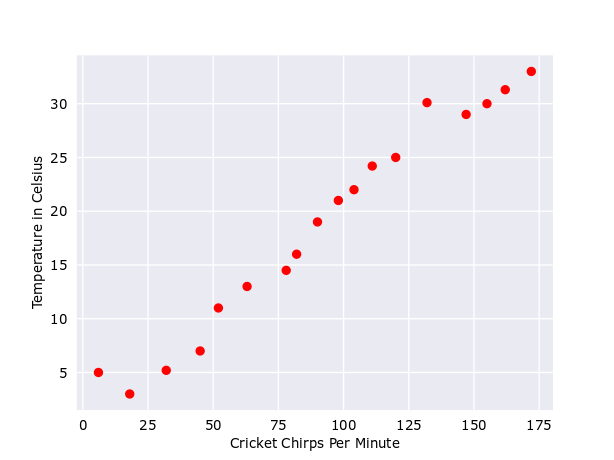
\includegraphics[width=0.8\textwidth]{images/CricketPoints.png}    
\end{itemize}
\end{frame}

%%%

\begin{frame}{Linear Regression}
\begin{itemize}
\item You could draw a single straight line like the following to approximate this relationship between chirps and temperature.

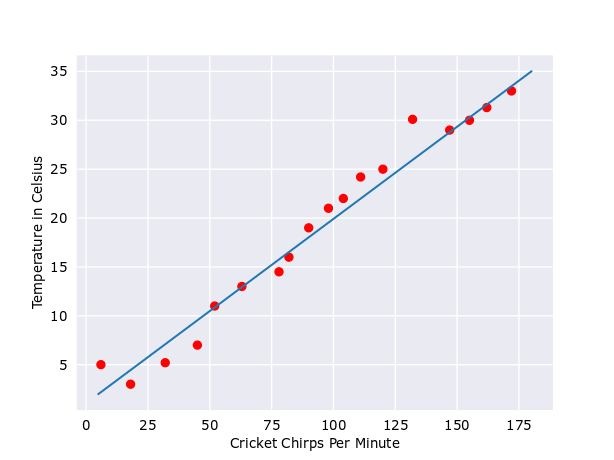
\includegraphics[width=0.8\textwidth]{images/CricketLine.png}    
\end{itemize}
\end{frame}

%%%

\begin{frame}{Linear Regression}
\begin{itemize}
\item The line doesn't pass through every dot, but the line does clearly show the relationship between chirps and temperature. 

\medskip
\item Using the equation for a line, you could write down this relationship as follows:
$$y = m x + b$$
where:

\medskip
\begin{itemize}
\item $y$ is the temperature in Celsius -- the value we're trying to predict.

\medskip
\item $m$ is the slope of the line.

\medskip
\item $x$ is the number of chirps per minute -- the value of our input feature.

\medskip
\item $b$ is the y-intercept.
\end{itemize}
\end{itemize}
\end{frame}

%%%

\begin{frame}{Linear Regression}
\begin{itemize}
\item By convention in ML, you'll write the equation for a model slightly differently:
$$\hat{y} = b + w_1 x_1$$

where:

\medskip
\begin{itemize}
\item $y$ is the predicted label (a desired output).

\medskip
\item $b$ is the bias (the $y$-intercept), sometimes referred to as $w_0$.

\medskip
\item $w_1$ is the weight of feature $1$. Weight is the same concept as the ``slope'' $m$ in the traditional equation of a line.

\medskip
\item $x_1$ is a feature (a known input).
\end{itemize}
\end{itemize}
\end{frame}

%%%

\begin{frame}{Linear Regression}
\begin{itemize}
\item To {\bf infer} (predict) the temperature $y'$ for a new chirps-per-minute value $x_1$, just substitute the $x_1$ value into this model.

\medskip    
\item Although this model uses only one feature, a more sophisticated model might rely on multiple features, each having a separate weight $w_1$, $w_2$, etc. 

\medskip    
\item For example, a model that relies on three features might look as follows:
$$ \hat{y} = b + w_1 x_1 + w_2 x_2 + w_3 x_3 $$
\end{itemize}
\end{frame}

%%%

\begin{frame}{Key Terms}
\begin{itemize}
    \item bias
    \item inference
    \item linear regression
    \item weight
\end{itemize}
\end{frame}

\end{document}